\chapter{Magnetic Inversion}\label{Chp:cook:magnetic inversion}

\begin{figure}
\centering
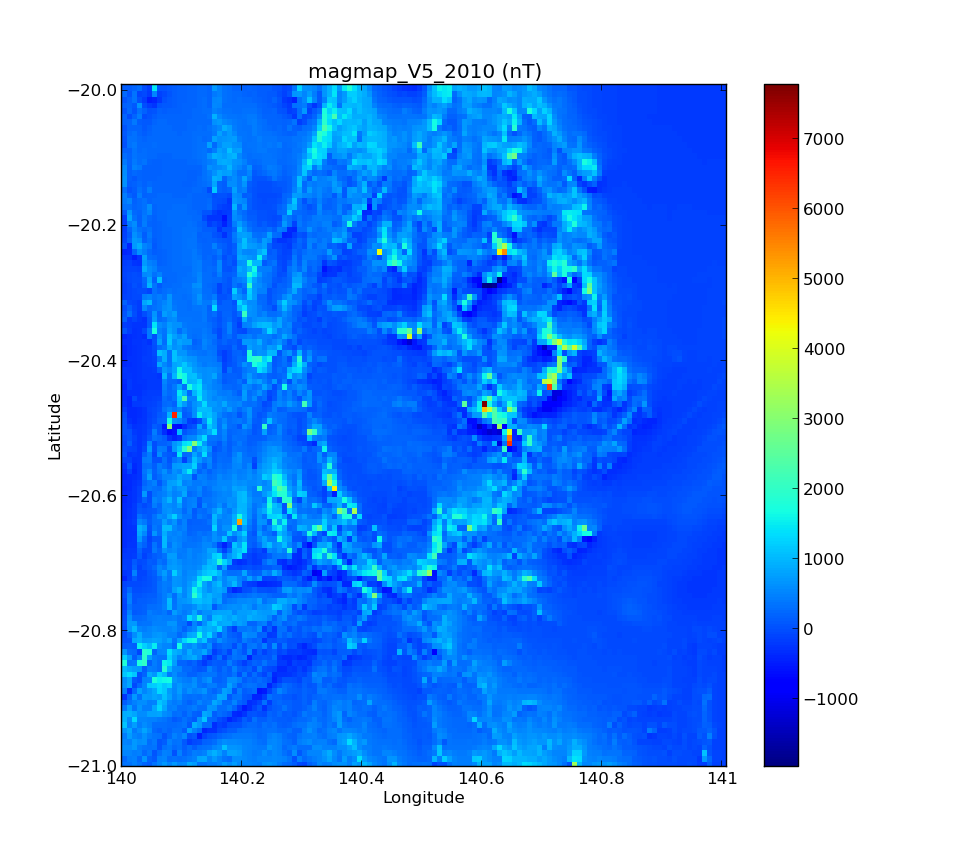
\includegraphics[width=0.7\textwidth]{QLDWestMagneticDataPlot.png}
\caption{Magnetic anomaly data in $nT$ from Western Queensland, Australia
    (file \examplefile{data/QLDWestMagnetic.nc}). Data obtained from Geoscience Australia.}
\label{FIG:P1:MAG:0}
\end{figure}

Magnetic data report the observed magnetic flux density over a region above the
surface of the Earth.
Similar to the gravity case the data are given as deviation from an expected
background magnetic flux density $B^b$ of the Earth.
Example data in units of $nT$ (nano Tesla) are shown in Figure~\ref{FIG:P1:MAG:0}.
It is the task of the inversion to recover the susceptibility distribution $k$
from the magnetic data collected. The approach for inverting magnetic data is
almost identical to the one used for gravity data. 
In fact the \downunder script~\ref{code: magnetic1} used for the magnetic
inversion is very similar to the script~\ref{code: gravity1} for gravity inversion.

\begin{pyc}\label{code: magnetic1}
\
\begin{python}
# Header:
from esys.downunder import *
from esys.weipa import *
from esys.escript import unitsSI as U


# Step 1: set up domain
dom=DomainBuilder()
dom.setVerticalExtents(depth=40.*U.km, air_layer=6.*U.km, num_cells=25)
dom.setFractionalPadding(pad_x=0.2, pad_y=0.2)
B_b = [2201.*U.Nano*U.Tesla,  31232.*U.Nano*U.Tesla, -41405.*U.Nano*U.Tesla]
dom.setBackgroundMagneticFluxDensity(B_b)
dom.fixSusceptibilityBelow(depth=40.*U.km)

# Step 2: read magnetic data
source0=NetCdfData(NetCdfData.MAGNETIC, 'MagneticSmall.nc', scale_factor=U.Nano * U.Tesla)
dom.addSource(source0)

# Step 3: set up inversion
inv=MagneticInversion()
inv.setSolverTolerance(1e-4)
inv.setSolverMaxIterations(50)
inv.fixMagneticPotentialAtBottom(False)
inv.setup(dom)

# Step 4: run inversion 
inv.getCostFunction().setTradeOffFactorsModels(0.1) 
k = inv.run()

# Step 5: write reconstructed susceptibility to file
saveVTK("result.vtu", susceptibility=k)
\end{python}
\end{pyc}

\begin{figure}
\centering
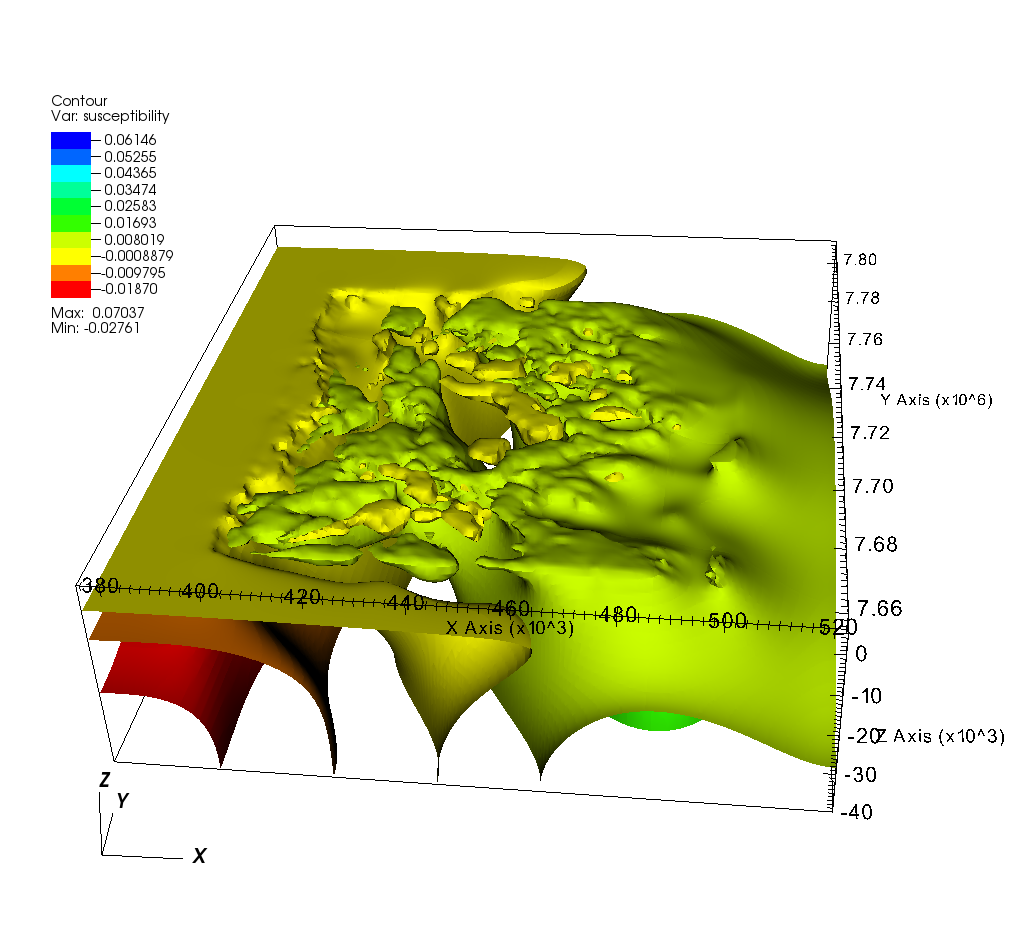
\includegraphics[width=0.7\textwidth]{QLDMagContourMu01.png}
\caption{Contour plot of the susceptibility from a three-dimensional magnetic inversion (with $\mu=0.1$).
Colours represent values of susceptibility where high values are represented by
    blue and low values are represented by red.}
\label{FIG:P1:MAG:1}
\end{figure}

The structure of the script is identical to the gravity case.
Following the header section importing the necessary modules the domain of the
inversion is defined in step one.
In step two the data are read and added to the domain builder.
Step three sets up the inversion and step four runs it.
Finally in step five the result is written to the result file, here
\file{result.vtu} in the \VTK format.
Results are shown in Figure~\ref{FIG:P1:MAG:1}.

Although scripts for magnetic and gravity inversion are largely identical there
are a few small differences which we are going to highlight now.
The magnetic inversion requires data about the background magnetic flux density
over the region of interest which is added to the domain by the statements 
\begin{verbatim}
B_b = [2201.*U.Nano*U.Tesla, 31232.*U.Nano*U.Tesla,  -41405.*U.Nano*U.Tesla]
dom.setBackgroundMagneticFluxDensity(B_b)
\end{verbatim}
Here it is assumed that the background magnetic flux density is constant across
the domain and is given as the list
\begin{verbatim}
B_b= [ B_E,  B_N, B_V ]
\end{verbatim}
in units of Tesla (T) where 
\member{B_N}, \member{B_E} and \member{B_V} refer to the north, east and
vertical component of the magnetic flux density, respectively.
Values for the magnetic flux density can be obtained by the International
Geomagnetic Reference Field (IGRF)~\cite{IGRF} (or the Australian Geomagnetic
Reference Field (AGRF)~\cite{AGRF} via \url{http://www.ga.gov.au/oracle/geomag/agrfform.jsp}).
Similar to the gravity case susceptibility below a certain depth can be set to
zero via the statement
\begin{verbatim}
dom.fixSusceptibilityBelow(depth=40.*U.km)
\end{verbatim}
where here the susceptibility below $40km$ is prescribed (this has no effect as
the depth of the domain is $40km$)\footnote{Notice that the method called is
different from the one in the case of gravity inversion.}. 

Magnetic data are read and added to the domain with the following statements:
\begin{verbatim}
source0=NetCdfData(NetCdfData.MAGNETIC, 'MagneticSmall.nc', \
                   scale_factor=U.Nano * U.Tesla)
dom.addSource(source0)
\end{verbatim}
The first argument \member{NetCdfData.MAGNETIC} identifies the data read from
file \file{MagneticSmall.nc} (second argument) as magnetic data.The argument
\file{scale_factor} specifies the units (here $nT$) of the magnetic flux
density data in the file.
If scalar data are given it is assumed that the magnetic flux density anomalies
are measured in direction of the background magnetic flux density\footnote{The
default for \file{scale_factor} for magnetic data is $nT$.}.

Finally the inversion is created and run:
\begin{verbatim}
inv=MagneticInversion()
inv.fixMagneticPotentialAtBottom(False)
k = inv.run()
\end{verbatim}
The result for the susceptibility is named \member{k}. In this case the magnetic potential is
not fixed at the bottom of the domain. The magnetic potential is still set zero at the top of the domain.

We then write the result
to a \VTK file using
\begin{verbatim}
saveVTK("result.vtu", susceptibility=k)
\end{verbatim}
where the result of the inversion is tagged with the name \member{susceptibility}
as an identifier for the visualization software. 

\begin{figure}
    \begin{center}
        \subfigure[$\mu=0.001$]{%
            \label{FIG:P1:MAG:10 MU0001}
            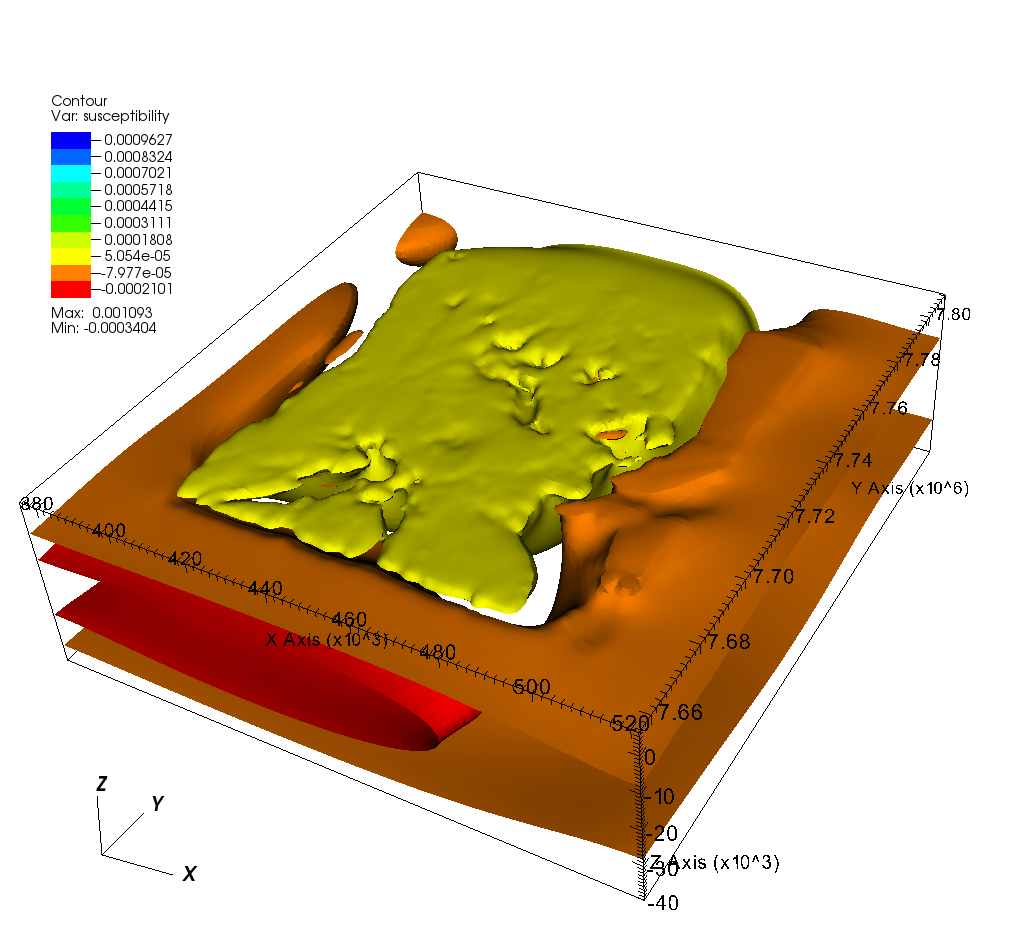
\includegraphics[width=0.45\textwidth]{QLDMagContourMu0001.png}
        }%
        \subfigure[$\mu=0.01$]{%
            \label{FIG:P1:MAG:10 MU001}
            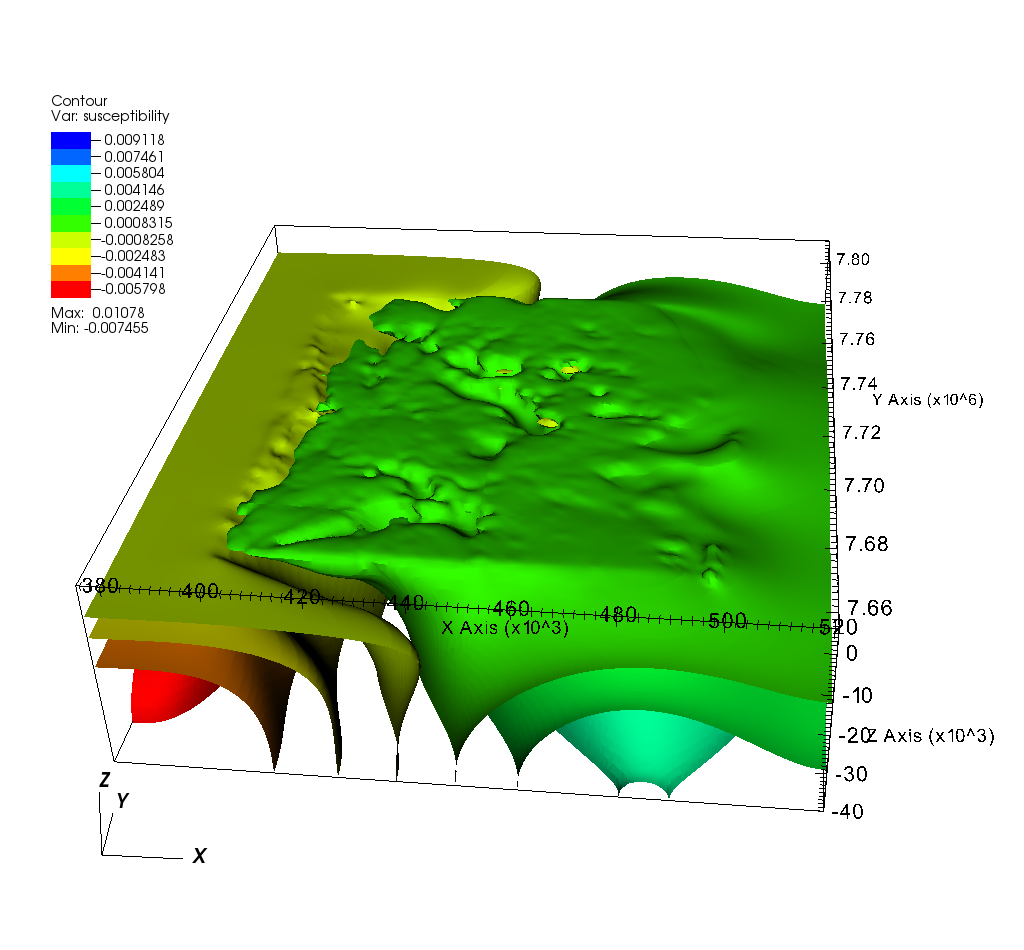
\includegraphics[width=0.45\textwidth]{QLDMagContourMu001.png}
        }\\ %  ------- End of the first row ----------------------%
        \subfigure[$\mu=0.1$]{%
            \label{FIG:P1:MAG:10 MU01}
            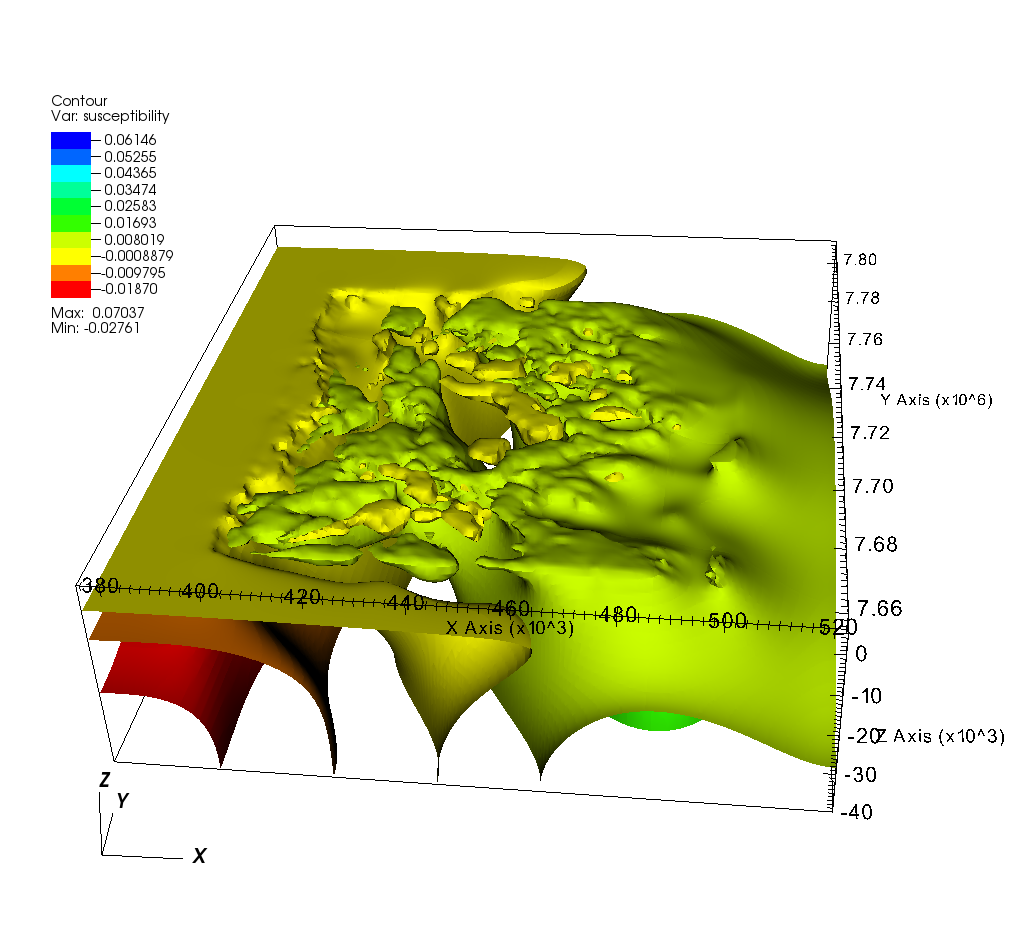
\includegraphics[width=0.45\textwidth]{QLDMagContourMu01.png}
        }%
        \subfigure[$\mu=1.$]{%
            \label{FIG:P1:MAG:10 MU1}
            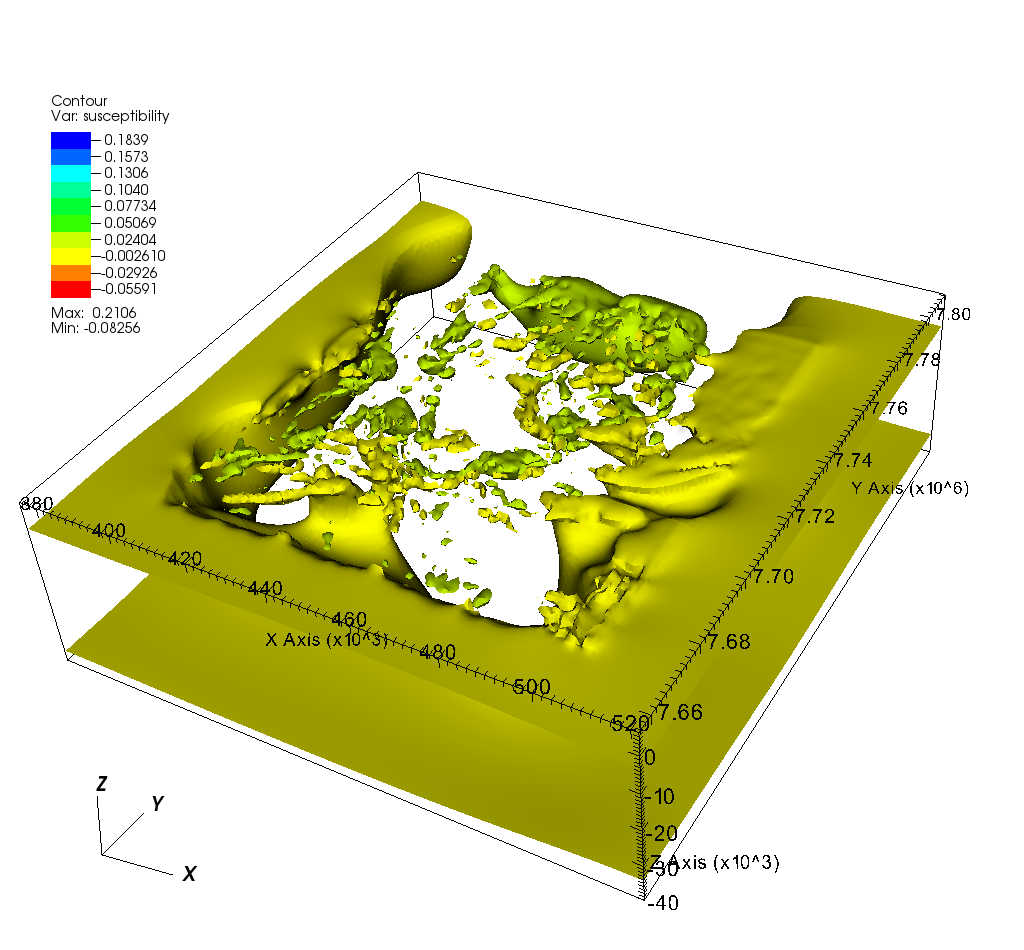
\includegraphics[width=0.45\textwidth]{QLDMagContourMu1.png}
        }\\ %  ------- End of the second row ----------------------%
        \subfigure[$\mu=10.$]{%
            \label{FIG:P1:MAG:10 MU10}
            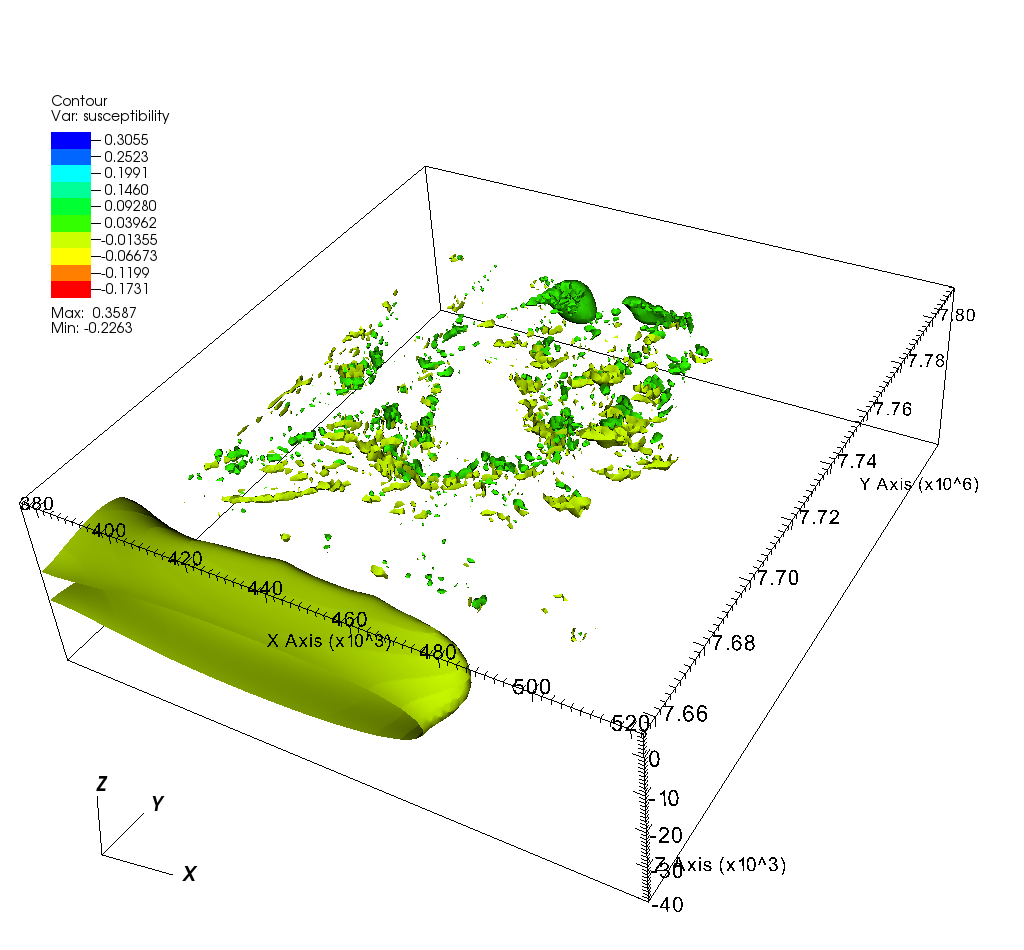
\includegraphics[width=0.45\textwidth]{QLDMagContourMu10.png}
        }%
    \end{center}
    \caption{3-D contour plots of magnetic inversion results with data from
    Figure~\ref{FIG:P1:MAG:0} for various values of the model trade-off
    factor $\mu$. Visualization has been performed in \VisIt.}
    \label{FIG:P1:MAG:10}
\end{figure}

\begin{figure}
    \begin{center}
        \subfigure[$\mu=0.001$]{%
            \label{FIG:P1:MAG:11 MU0001}
            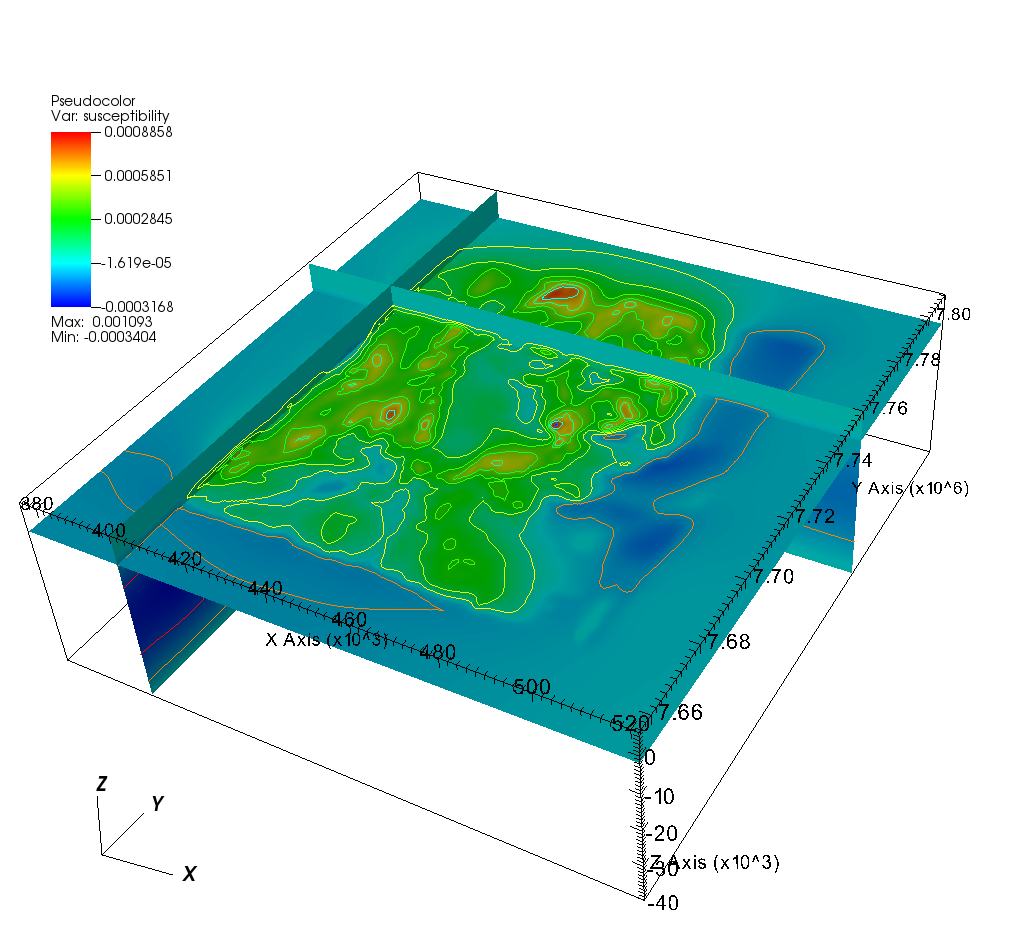
\includegraphics[width=0.45\textwidth]{QLDMagDepthMu0001.png}
        }%
        \subfigure[$\mu=0.01$]{%
            \label{FIG:P1:MAG:11 MU001}
            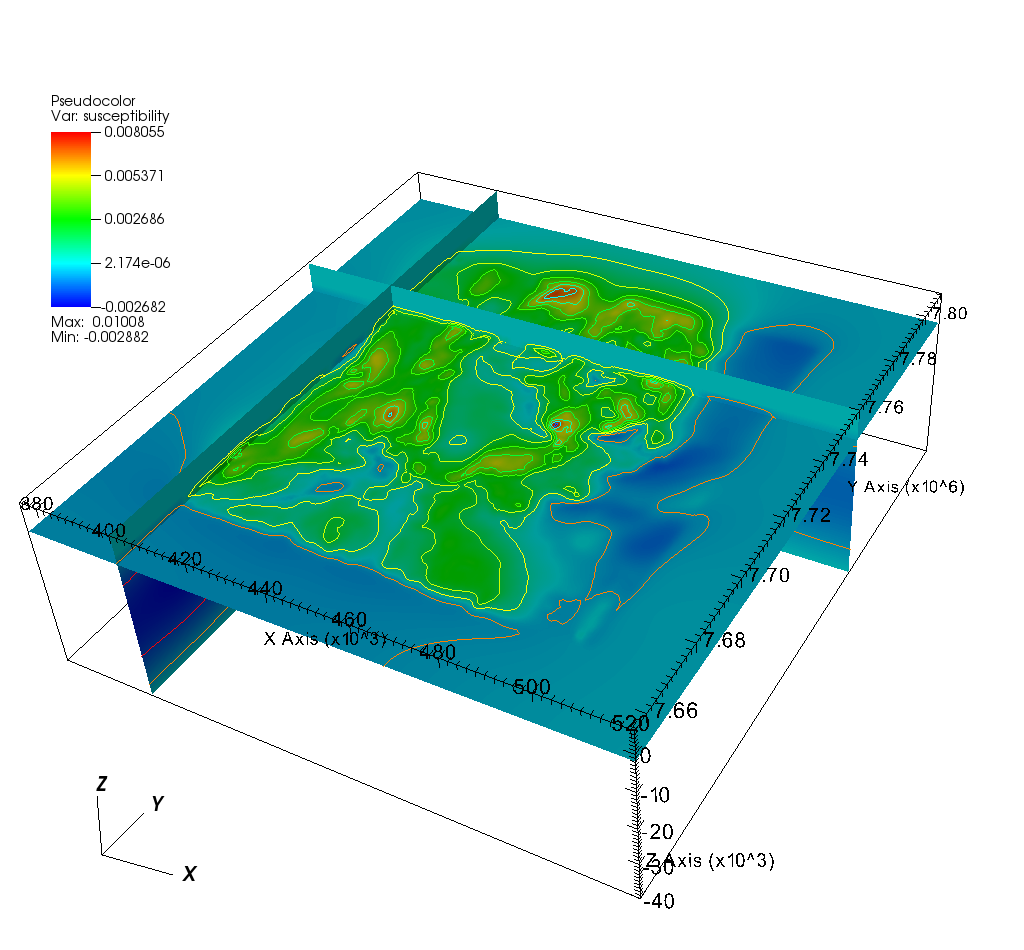
\includegraphics[width=0.45\textwidth]{QLDMagDepthMu001.png}
        }\\ %  ------- End of the first row ----------------------%
        \subfigure[$\mu=0.1$]{%
            \label{FIG:P1:MAG:11 MU01}
            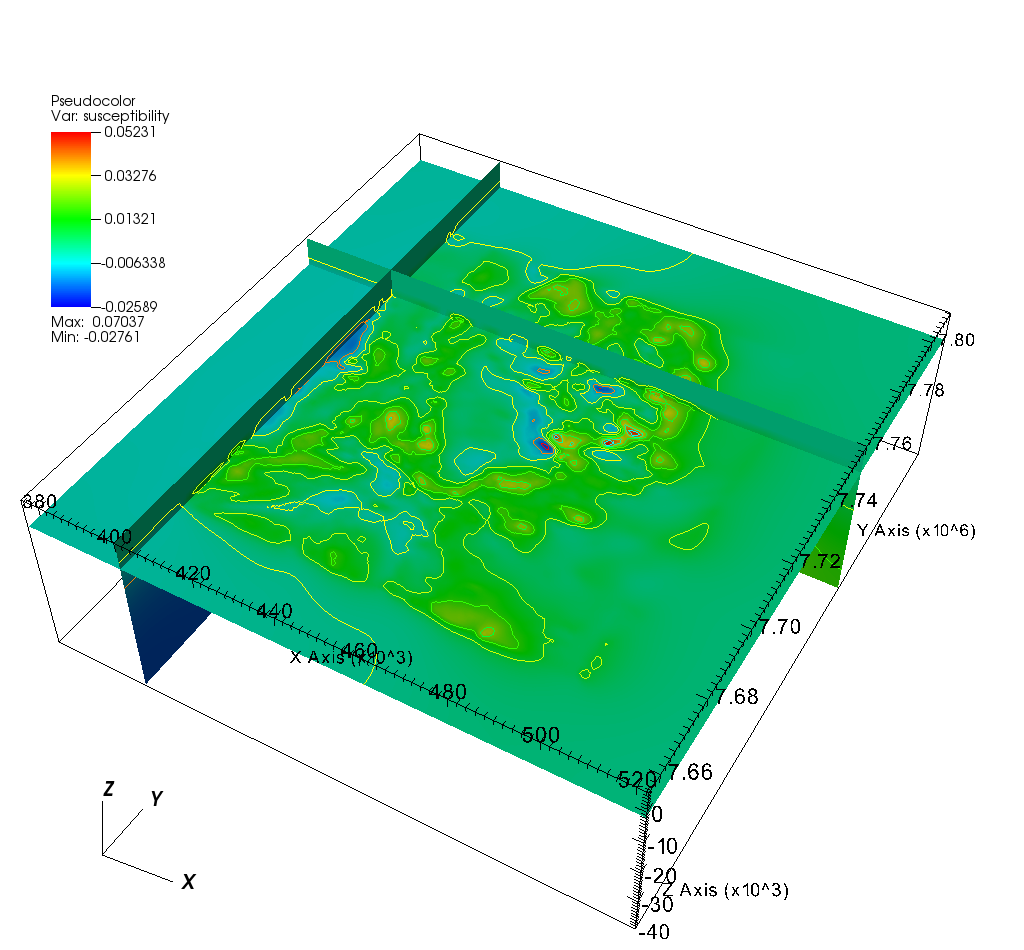
\includegraphics[width=0.45\textwidth]{QLDMagDepthMu01.png}
        }%
        \subfigure[$\mu=1.$]{%
            \label{FIG:P1:MAG:11 MU1}
            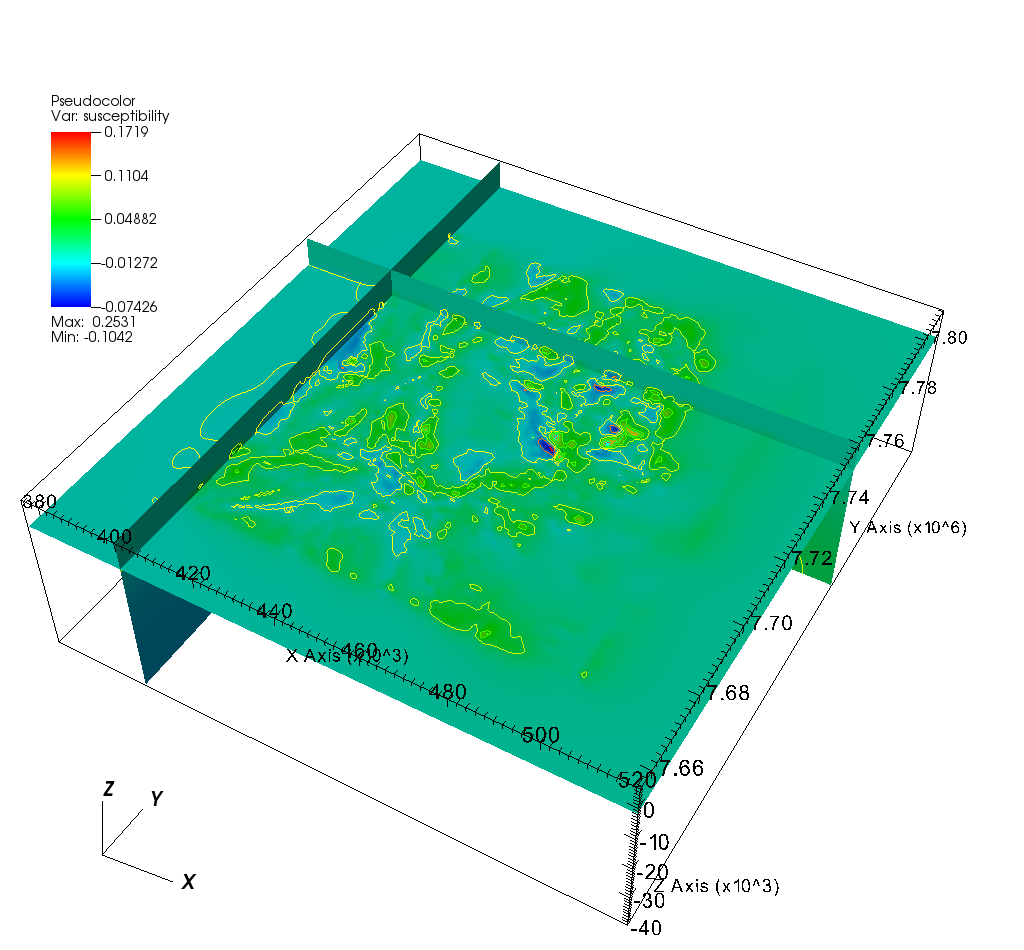
\includegraphics[width=0.45\textwidth]{QLDMagDepthMu1.png}
        }\\ %  ------- End of the second row ----------------------%
        \subfigure[$\mu=10.$]{%
            \label{FIG:P1:MAG:11 MU10}
            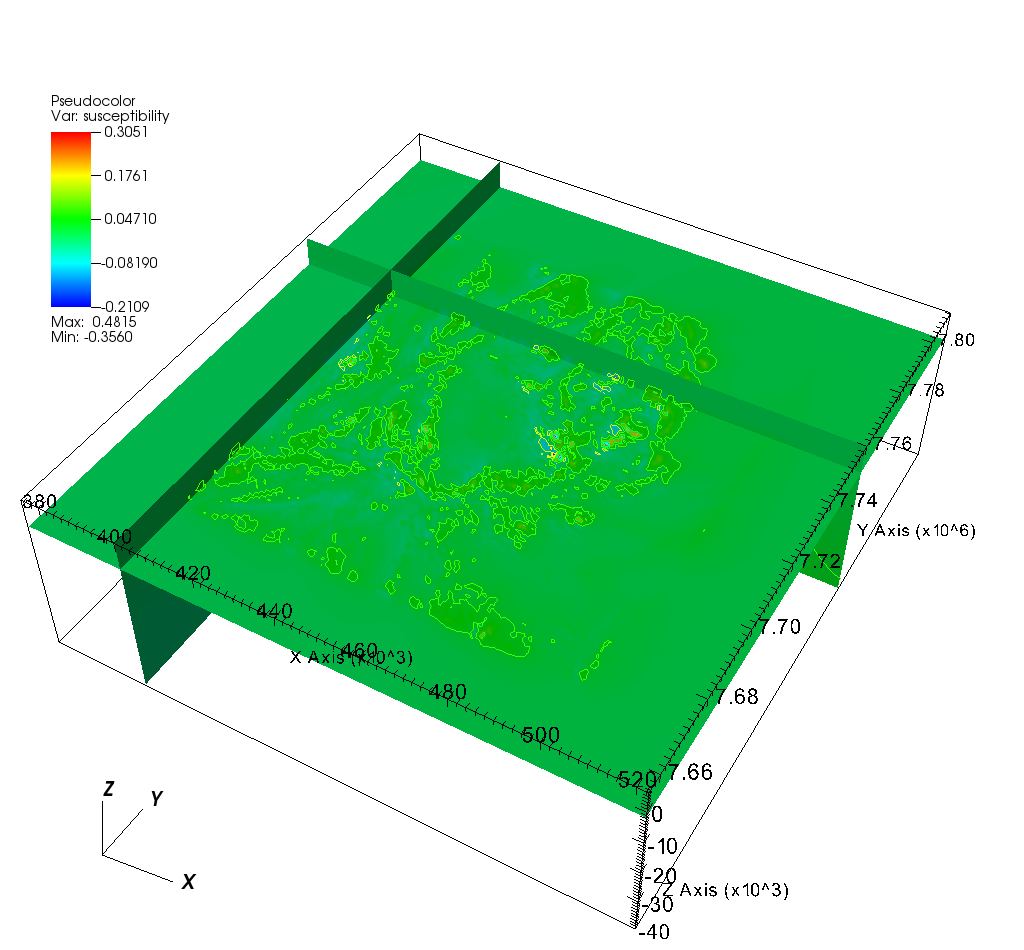
\includegraphics[width=0.45\textwidth]{QLDMagDepthMu10.png}
        }%
    \end{center}
    \caption{3-D slice plots of magnetic inversion results with data from
    Figure~\ref{FIG:P1:MAG:0} for various values of the model trade-off
    factor $\mu$. Visualization has been performed \VisIt.}
    \label{FIG:P1:MAG:11}
\end{figure}

Figures~\ref{FIG:P1:MAG:10} and~\ref{FIG:P1:MAG:11} show results from the
inversion of the magnetic data shown in Figure~\ref{FIG:P1:MAG:0}.
In Figure~\ref{FIG:P1:MAG:10} surface contours are used to represent the
susceptibility while Figure~\ref{FIG:P1:MAG:11} uses contour lines
on a lateral plane intercept and two vertical plane intercepts.
The images show the strong impact of the trade-off factor $\mu$ on the result.
Larger values give more emphasis to the misfit term in the cost function
leading to rougher susceptibility distributions.
The result for $\mu=0.1$ seems to be the most realistic.

